\part{Capítulo nueve}

\graphicspath{ {9_Capitulo/img/ejemplos/},{9_Capitulo/img/explicacion/}, {W_Varios/2_Portada_capitulos/} }

%----------------------------------------------------------------------------------------
%	CHAPTER 9

\chapter{Valor presente neto}
\section{Mapa Mental}
\begin{center}
	\includegraphics[width=16cm]{Mapa Mental 9.pdf}
\end{center}
\section{Fórmulas del capítulo}

\begin{spacing}{1.5}
	\begin{center}
		\begin{tabular}{ |p{6cm}|p{5cm}| p{4cm}|}
			\hline
			\rowcolor{orange!50}
			\begin{center}\textbf{Fórmula} \end{center}   & \begin{center} \textbf{Nombre}\end{center} & \begin{center} \textbf{Excel} \end{center} \\ \hline
			
			VPN =	$\sum F_{n}(1+i)^{-n}$ & Valor Presente Neto       & -                         \\ \hline
		\end{tabular}
	\end{center}
\end{spacing}

\section{Introducción}

Es indispensable evaluar un proyecto de inversión financieramente previo a relizarlo, para determinar si es aconsejable o no. Por tal motivo se estudiará el concepto y aplicación de índices tales como: El VPN, el CAUE, la TIR, la relación beneficio costo, el VPNE, el PPA, etc.

\section{VALOR PRESENTE NETO}
El valor presente neto, VPN, es el más utilizado; pone en pesos de hoy tanto  ingresos como egresos futuros, facilitando la toma de decisiones desde el punto de vista financiero.
Si el $VPN > 0$ el proyecto es rentable, en pesos de hoy, los ingresos son mayores que los egresos; si el $VPN < 0$ significa que en pesos de hoy los ingresos son menores que los egresos y por lo tanto el proyecto no debería realizarse y, si el VPN = 0 COP tanto ingresos como egresos serán iguales, denotando que financieramente le será indiferente al inversionista.
Desde el punto de vista matemático el VPN es la sumatoria de los flujos de caja puestos en el día de hoy, lo cual podemos representar por:
\begin{center}
	VPN =	$\sum F_{n}(1+i)^{-n}$
\end{center}
\section{Definición de tasa de interés de oportunidad (TIO)}
La tasa de interés de oportunidad (TIO) es la tasa de interés más alta que un inversionista sacrifíca con el objeto de realizar un proyecto.
La definición anterior la podemos explicar mediante el siguiente ejemplo: Supongamos que el inversionista A tiene las siguientes posibilidades para invertir su dinero:
\begin{enumerate}[label=\alph*)]
	\item Comprar una maquina que le producirá una rentabilidad del 3\% mensual.
	\item Prestar el dinero a un amigo que le pagará con un interés del 2.5 \% mensual.
	\item Invertir en sus negocios normales, los cuales le dan una rentabilidad del 2.8\% mensual.
	\item Invertir en una cuenta de ahorros que paga al 1.5\% mensual.
	\item Invertir en un CDT, donde se le garantiza el 2\% mensual.
\end{enumerate}
El inversionista B solo tiene dos posibilidades.
\begin{enumerate}[label=\alph*)]
	\item Invertir en la cuenta de ahorros con una rentabilidad del 1.5\% mensual.
	\item Invertir en un CDT, donde se le garantiza el 2\% mensual.
\end{enumerate}
De acuerdo con el planteamiento anterior; para el inversionista A, la TIO es del 3\% mensual y para el inversionista B, la TIO será del 2\% mensual.
\\
\\
\textbf{Ejemplo 1}\\
Para realizar un proyecto se necesita realizar una inversión inicial de 80.000 COP y otra inversión de
45.000 COP al final del primer mes, en los meses 2 y 3 los ingresos son equivalentes a los egresos;
pero a partir del mes 4, se producen ingresos así: Mes cuatro 30.000 COP, mes cinco 50.000 COP, mes
seis 60.000 COP. Determinar si el proyecto lo pueden realizar los inversionistas A o B mencionados
anteriormente.\\


%%%%%%%%%%%%%%%%%%% EJERCICIO 1 %%%%%%

%\newpage %USAR SOLO SI EL SOLUCION QUEDA SOLO Y ES NECESARIO BAJARLO A LA SIGUIENTE PAGINA
\textbf{Solución.}\\
%La tabla ira centrada
\begin{center}
	\renewcommand{\arraystretch}{1.5}% Margenes de las celdas
	%Creacion de la cuadricula de 3 columnas \end{flushleft}
	\begin{longtable}[H]{|C{0.3\linewidth}|C{0.3\linewidth}|C{0.3\linewidth}|}
		%Creamos una linea horizontal
		\hline
         %%%%% INICIO FLUJO DE CAJA
		\rowcolor[HTML]{FFB183}
		\multicolumn{3}{|c|}{\cellcolor[HTML]{FFB183}\textbf{1. Asignación periodo focal}}   \\ \hline
		\multicolumn{3}{|c|} {$pf = 0 pmv$} \\ \hline
		%%%%%%%%%% FIN TITULO
		%%%%%%%%%% INICIO TITULO
		%Lo que se hace aqui es mezclar las 3 columnas en una sola
		\multicolumn{3}{|c|}{\cellcolor[HTML]{FFB183}\textbf{2. Declaración de variables}}   \\ \hline
		%%%%%%%%%% FIN TITULO
		%%%%%%%%%% INICIO DE MATEMATICAS
		%Cada & hace referencia al paso de la siguiente columna
		$n_{0} = 0 pmv$   & $n_{1} = 1 pmv$ & $n_{2} =  4 pmv$\\
		$n_{3} = 5 pmv$ & $n_{4} = 6 pmv$ & \\ \hline
		\multicolumn{3}{|c|}{$i_{a} = TIO_{a} = 3\% \equiv 0.03 pmv$} \\
		\multicolumn{3}{|c|}{$i_{b} = TIO_{b} = 2\% \equiv 0.02 pmv$} \\ \hline
		%%%%%%%%%% FIN DE MATEMATICAS
		%%%%% FIN DECLARACION DE VARIABLES


		%%%%% INICIO FLUJO DE CAJA
		\rowcolor[HTML]{FFB183}
		\multicolumn{3}{|c|}{\cellcolor[HTML]{FFB183}\textbf{3. Diagrama de flujo de caja}} \\ \hline
		%Mezclamos 3 columnas y ponermos el dibujo
		%%%%%%%%%%%%% INSERCION DE LA IMAGEN
		%Deberan descargar las imagenes respectivas del drive y pegarlas en la carpeta
		%n_capitulo/img/ejemplos/1/capitulo1ejemplo1.pdf  (el /1/ es el numero del ejemplo)
		\multicolumn{3}{|c|}{ 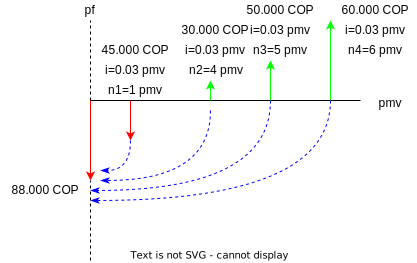
\includegraphics[trim=-5 -5 -5 -5 , scale=1.0,width=300px, height=250px]{9_Capitulo/ejemplos/1/Capitulo9Ejercicio1.pdf} }   \\ \hline
		%%%%%%%%%%%%% FIN INSERCION DE IMAGEN
		%%%%%FIN FLUJO DE CAJA



		%%%%% INICIO DECLARACION FORMULAS
		%%%%%%%%%%% INICIO TITULO
		\rowcolor[HTML]{FFB183}
		\multicolumn{3}{|c|}{\cellcolor[HTML]{FFB183}\textbf{4. Declaración de fórmulas}}    \\ \hline
		%%%%%%%%%%% FIN TITULO
		%%%%%%%%%%% INICIO MATEMATICAS
		\multicolumn{3}{|c|}{$\sum F_{n}(1+i)^{-n} $\hspace{0.3cm} \textit{Valor presente neto}} \\ \hline
		%%%%%%%%%% FIN MATEMATICAS
		%%%%%% INICIO DESARROLLO MATEMATICO
		\rowcolor[HTML]{FFB183}
		%%%%%%%%%%INICIO TITULO
		\multicolumn{3}{|c|}{\cellcolor[HTML]{FFB183}\textbf{5. Desarrollo matemático}}       \\ \hline
		%%%%%%%%%% FIN TITULO
		%%%%%%%%%% INICIO MATEMATICAS
		\multicolumn{3}{|c|}{$VPN_{a} = -80000 - 45000(1+0.03)^{-1} + 30000(1+0.03)^{-4} + 50000(1+0.03)^{-5} + 60000(1+0.03)^{-6}$} \\
		\multicolumn{3}{|c|}{$VPN_{a} = -3655$} \\
		\multicolumn{3}{|c|}{$VPN_{b} = -80000 - 45000(1+0.02)^{-1} + 30000(1+0.02)^{-4} + 50000(1+0.02)^{-5} + 60000(1+0.02)^{-6}$} \\
		\multicolumn{3}{|c|}{$VPN_{b} = 216254$} \\ \hline

		%%%%%%%%%% FIN MATEMATICAS
		%%%%%% FIN DESARROLLO MATEMATICO
		%%%%%% INICIO RESPUESTA
		\rowcolor[HTML]{FFB183}
		%%%%%%%%%%INICIO TITULO
		\multicolumn{3}{|c|}{\cellcolor[HTML]{FFB183}\textbf{6. Respuesta}}   \\ \hline
		%%%%%%%%%% FIN TITULO
		%%%%%%%%%% INICIO RESPUESTA MATEMATICA
		\multicolumn{3}{|c|}{Para B el $VPN > 0$, significa que puede realizar el proyecto en pesos de hoy,} \\ 
		\multicolumn{3}{|c|}{además de ganarse el 2\%, obtiene una ganancia de 2.162,54 COP.}  \\ \hline
		%%%%%%%%%% FIN MATEMATICAS
		%%%%%% FIN RESPUESTA
	\end{longtable}
	%Se crean dos lineas en blanco para que no quede el siguiente texto tan pegado
	%\newline \newline %USARLO SI CREES QUE ES NECESARIO
\end{center}
%%%%%%%%%%%%%%%%%%%%%%%%%%FIN EJERCICIO 1 %%%%%%%%%%%%%%%%%%%%%%%%%%%


\section{Símbolos.}

Con el fin de facilitar la construcción de gráficas y, para simplificar la escritura, adoptaremos los siguientes símbolos.\\

C0  =  Costo inicial o inversión inicial.\\
C1  =  Costos en el período 1 o inversión en el periodo 1.\\
C2  =  Costos en el período 2 o inversión en el periodo 2.\\
.\\
.\\
.\\
Cn  =  Costo en el período n o inversión en el periodo n.\\
K  =  Vida útil (expresada en años, en meses o en unidades producidas).\\
S  =  Valor de salvamento.\\
CAO  =  Costo anual de operación o serie neta uniforme de costo de operación, cuando los costos son mensuales se representará por CMO.\\
I1  =  Ingreso en el período 1.\\
I2  =  Ingreso en el período 2.\\
.\\
.\\
.\\
In  =  Ingreso del período n.\\

\section{UTILIZACIÓN DEL VPN}

El VPN puede utilizarse en proyectos individuales o en la decisión sobre alternativas de inversión; en el primer caso, solo basta conocer el signo del VPN para tomar una decisión; como se puede apreciar en el siguiente ejemplo.\\
\\
\textbf{Ejemplo 2}\\
Se invierten 200{.}000 COP en un depósito a término fijo de 6 meses en un banco que paga el 28\% namv. Determinar el monto de la entrega al vencimiento.\\

%%%%%%%%%%%%%%%%%%% EJERCICIO 1 %%%%%%

%\newpage %USAR SOLO SI EL SOLUCIÓN QUEDA SOLO Y ES NECESARIO BAJARLO A LA SIGUIENTE PAGINA
\textbf{Solución.}
%La tabla ira centrada
\begin{center}
  \renewcommand{\arraystretch}{1.5}% Margenes de las celdas
  %Creación de la cuadricula de 3 columnas \end{flushleft}
  \begin{longtable}[H]{|C{0.3\linewidth}|C{0.3\linewidth}|C{0.3\linewidth}|}
    %Creamos una linea horizontal
    \hline
    %Definimos el color de la primera fila
    \rowcolor[HTML]{FFB183}
    %%%%% INICIO ASIGNACIÓN FECHA FOCAL %%%%%%%
    %%%%%%%%%% INICIO TITULO
    %Lo que se hace aquí es mezclar las 3 columnas en una sola
    \multicolumn{3}{|c|}{\cellcolor[HTML]{FFB183}\textbf{1. Asignación período focal}}                                  \\ \hline
    %%%%%%%%%% FIN TITULO
    %%%%% INICIO DECLARACIÓN DE VARIABLES %%%%%%%
    \multicolumn{3}{|c|}{$pf = 6pmv$}                                                                                   \\ \hline
    %%%%%%%%%% INICIO TITULO
    %Lo que se hace aquí es mezclar las 3 columnas en una sola
    \multicolumn{3}{|c|}{\cellcolor[HTML]{FFB183}\textbf{2. Declaración de variables}}                                  \\ \hline
    %%%%%%%%%% FIN TITULO
    %%%%%%%%%% INICIO DE MATEMÁTICAS
    %Cada & hace referencia al paso de la siguiente columna
    $P =  200{.}000$ COP & $n = 6\textit{pmv} $ & $i= ?\% pmv$                                                           \\
    $j=28\%namv$         & $m=12pmv$            & $F = ? COP$                                                           
    \\\hline

    %%%%%%%%%% FIN DE MATEMÁTICAS
    %%%%% FIN DECLARACIÓN DE VARIABLES


    %%%%% INICIO FLUJO DE CAJA
    \rowcolor[HTML]{FFB183}
    \multicolumn{3}{|c|}{\cellcolor[HTML]{FFB183}\textbf{3. Diagrama de flujo de caja}}                                 \\ \hline
    %Mezclamos 3 columnas y pondremos el dibujo
    %%%%%%%%%%%%% INSERCIÓN DE LA IMAGEN
    %Deberán descargar las imágenes respectivas del drive y pegarlas en la carpeta
    %n_capitulo/img/ejemplos/1/capitulo1ejemplo1.pdf  (el /1/ es el numero del ejemplo)
    \multicolumn{3}{|c|}{ 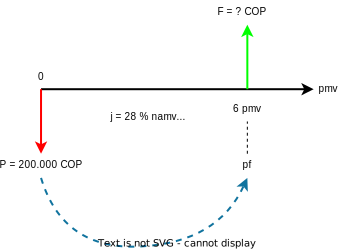
\includegraphics[trim=-5 -5 -5 -5 , scale=1]{2_Capitulo/ejemplos/2/Capitulo2Ejercicio2_v2.pdf} } \\ \hline
    %%%%%%%%%%%%% FIN INSERCIÓN DE IMAGEN
    %%%%%FIN FLUJO DE CAJA



    %%%%% INICIO DECLARACIÓN FORMULAS
    %%%%%%%%%%% INICIO TITULO
    \rowcolor[HTML]{FFB183}
    \multicolumn{3}{|c|}{\cellcolor[HTML]{FFB183}\textbf{4. Declaración de fórmulas}}                                   \\ \hline
    %%%%%%%%%%% FIN TITULO
    %%%%%%%%%%% INICIO MATEMÁTICAS
    \multicolumn{3}{|c|}{$F = P(1+i)^n \hspace{0.3cm} \textit{Valor futuro}$}                                           \\
    \multicolumn{3}{|c|}{$j=i\cdot m\hspace{0.3cm}\textit{Tasa periódica anualizada}$}
    \\ \hline
    %%%%%%%%%% FIN MATEMÁTICAS
    %%%%%% INICIO DESARROLLO MATEMÁTICO
    \rowcolor[HTML]{FFB183}
    %%%%%%%%%%INICIO TITULO
    \multicolumn{3}{|c|}{\cellcolor[HTML]{FFB183}\textbf{5. Desarrollo matemático}}                                     \\ \hline
    %%%%%%%%%% FIN TITULO
    %%%%%%%%%% INICIO MATEMÁTICAS
    \multicolumn{3}{|c|}{$0{.}28=i\cdot 12$}                                                                            \\
    \multicolumn{3}{|c|}{$i= \frac{0{.}28}{12} = 0{.}02333... \equiv 2{.}333\%pmv$}                                     \\
    \multicolumn{3}{|c|}{$0{.}28=i\cdot 12$}                                                                            \\
    \multicolumn{3}{|c|}{$F = 200{.}000 COP(1+0,2333)^6$}                                                       \\
    \multicolumn{3}{|c|}{$F = 229{.}685.04 COP$}
    \\ \hline


    %%%%%%%%%% FIN MATEMÁTICAS
    %%%%%% FIN DESARROLLO MATEMÁTICO
    %%%%%% INICIO RESPUESTA
    \rowcolor[HTML]{FFB183}
    %%%%%%%%%%INICIO TITULO
    \multicolumn{3}{|c|}{\cellcolor[HTML]{FFB183}\textbf{6. Respuesta}}                                                 \\ \hline
    %%%%%%%%%% FIN TITULO
    %%%%%%%%%% INICIO RESPUESTA MATEMÁTICA
    \multicolumn{3}{|c|}{$F = 229{.}685.04 COP$
    }                                                                                                                   \\ \hline
    %%%%%%%%%% FIN MATEMÁTICAS
    %%%%%% FIN RESPUESTA
  \end{longtable}
  %Se crean dos lineas en blanco para que no quede el siguiente texto tan pegado
  %\newline \newline %USARLO SI CREES QUE ES NECESARIO
\end{center}
%%%%%%%%%%%%%%%%%%%%%%%%%%FIN EJERCICIO 1 %%%%%%%%%%%%%%%%%%%%%%%%%%%


\section{ALTERNATIVAS MUTUAMENTE EXCLUYENTES}

Puede ocurrir que simultáneamente se presenten varios proyectos, pera la ejecución de uno de ellos excluye la posibilidad de ejecución de cualquiera de los otros, en este caso se debe evaluar cada alternativa por separado, pero siempre usando el mismo horizonte de planeación a fin de poderlos comparar.\\
\\
\textbf{Ejemplo 3}\\
Una fabrica produce actualmente en forma manual 1.000 unidades de un determinado artículo, para ello utiliza artesanos a los cuales les paga 8.400.000 COP al año y, es costumbre que cada año se les aumente el sueldo en aproximadamente un 20\%. El precio de venta de cada artículo es de 9.000 COP y se estima que este precio podrá ser aumentado todos los años en un 21\%. Ahora se ha presentado la oportunidad de adquirir una máquina a un costo de 10 millones COP con una vida útil de 5 años; un valor de salvamento de 2 millones COP la cual requiere de 2 técnicos para su operación, el sueldo anual de cada uno de los técnicos puede ser de 600.000 COP con aumentos anuales de sueldo del 20\% ¿Cuál de las dos alternativas es mejor suponiendo que la tasa del inversionista es del 30\%?\\


%%%%%%%%%%%%%%%%%%% EJERCICIO 3 %%%%%%

%\newpage %USAR SOLO SI EL SOLUCION QUEDA SOLO Y ES NECESARIO BAJARLO A LA SIGUIENTE PAGINA
\textbf{Solución.}\\
%La tabla ira centrada
\begin{center}
	\renewcommand{\arraystretch}{1.5}% Margenes de las celdas
	%Creacion de la cuadricula de 3 columnas \end{flushleft}
	\begin{longtable}[H]{|C{0.3\linewidth}|C{0.3\linewidth}|C{0.3\linewidth}|}
		%Creamos una linea horizontal
		\hline
        %%%%% INICIO FLUJO DE CAJA
		\rowcolor[HTML]{FFB183}
		\multicolumn{3}{|c|}{\cellcolor[HTML]{FFB183}\textbf{1. Asignación periodo focal}}   \\ \hline
		\multicolumn{3}{|c|} {$pf = 0 pav$} \\ \hline
		%%%%%%%%%% FIN TITULO
		%%%%%%%%%% INICIO TITULO
		%Lo que se hace aqui es mezclar las 3 columnas en una sola
		\multicolumn{3}{|c|}{\cellcolor[HTML]{FFB183}\textbf{2. Declaración de variables}}   \\ \hline
		%%%%%%%%%% FIN TITULO
		%%%%%%%%%% INICIO DE MATEMATICAS
		%Cada & hace referencia al paso de la siguiente columna
		$R_{1} = 9.000.000 $ COP   & $R_{2} = 8.400.000$ COP  & $i=0.3pav$\\ 
		$g_{1} =  0.21 pav $ & $g_{2}=  0.2 pav $ & $n=5pav$ \\ \hline
		%%%%%%%%%% FIN DE MATEMATICAS
		%%%%% FIN DECLARACION DE VARIABLES

  		%%%%% INICIO DECLARACION FORMULAS
  
		%%%%%%%%%%% INICIO TITULO
		\rowcolor[HTML]{FFB183}
		\multicolumn{3}{|c|}{\cellcolor[HTML]{FFB183}\textbf{3. Diagrama de flujo de caja}} \\ \hline
		%Mezclamos 3 columnas y ponermos el dibujo
		%%%%%%%%%%%%% INSERCION DE LA IMAGEN
		%Deberan descargar las imagenes respectivas del drive y pegarlas en la carpeta
		%n_capitulo/img/ejemplos/1/capitulo1ejemplo1.pdf  (el /1/ es el numero del ejemplo)
		\multicolumn{3}{|c|}{ \includegraphics[trim=-5 -5 -5 -5 , scale=1, width=300px, height=250px]{9_Capitulo/ejemplos/3/Capitulo9Ejercicio3.pdf} }   \\ \hline
		%%%%%%%%%%%%% FIN INSERCION DE IMAGEN
		%%%%%FIN FLUJO DE CAJA



		%%%%% INICIO DECLARACION FORMULAS
		%%%%%%%%%%% INICIO TITULO
		\rowcolor[HTML]{FFB183}
		\multicolumn{3}{|c|}{\cellcolor[HTML]{FFB183}\textbf{4. Declaración de fórmulas}}    \\ \hline
		%%%%%%%%%%% FIN TITULO
		%%%%%%%%%%% INICIO MATEMATICAS
		\multicolumn{3}{|c|}{$\sum F_{n}(1+i)^{-n} $\hspace{0.3cm} \textit{Valor presente neto}} \\ \hline
		%%%%%%%%%% FIN MATEMATICAS
		%%%%%% INICIO DESARROLLO MATEMATICO
		\rowcolor[HTML]{FFB183}
		%%%%%%%%%%INICIO TITULO
		\multicolumn{3}{|c|}{\cellcolor[HTML]{FFB183}\textbf{5. Desarrollo matemático}}       \\ \hline
		%%%%%%%%%% FIN TITULO
		%%%%%%%%%% INICIO MATEMATICAS
		\multicolumn{3}{|c|}{$VPN_{A} = \frac{9[(1+0.21)^{5}(1+0.3)^{-5} -1]}{0.21-0.3} - \frac{8.4[(1+0.2)^{5}(1+0.3^{-5} -1)]}{0.2-0.3}$} \\
		\multicolumn{3}{|c|}{$VPN_{A} = 2.437.836 $ COP} \\
		\multicolumn{3}{|c|}{$VPN_{B} = \frac{9[(1+0.21)^{5}(1+0.3)^{-5} -1]}{0.21-0.3} + 2(1.3)^{-5} - \frac{1.2[(1+0.2)^{5}(1+0.3^{-5} -1)]}{0.2-0.3}$} \\
		\multicolumn{3}{|c|}{$VPN_{B} = 16.723.756 $ COP} \\ \hline

		%%%%%%%%%% FIN MATEMATICAS
		%%%%%% FIN DESARROLLO MATEMATICO
		%%%%%% INICIO RESPUESTA
		\rowcolor[HTML]{FFB183}
		%%%%%%%%%%INICIO TITULO
		\multicolumn{3}{|c|}{\cellcolor[HTML]{FFB183}\textbf{6. Respuesta}}   \\ \hline
		%%%%%%%%%% FIN TITULO
		%%%%%%%%%% INICIO RESPUESTA MATEMATICA
		\multicolumn{3}{|c|}{La decisión correcta es comprar la máquina.}  \\ \hline
		%%%%%%%%%% FIN MATEMATICAS
		%%%%%% FIN RESPUESTA
	\end{longtable}
	%Se crean dos lineas en blanco para que no quede el siguiente texto tan pegado
	%\newline \newline %USARLO SI CREES QUE ES NECESARIO
\end{center}
%%%%%%%%%%%%%%%%%%%%%%%%%%FIN EJERCICIO 3 %%%%%%%%%%%%%%%%%%%%%%%%%%%


\section{ALTERNATIVAS MUTUAMENTE EXCLUYENTES CON DIFERENTE VIDA ÚTIL}

Dado que el VPN exige que el horizonte planeación sea de igual número de períodos en cada alternativa y, en éste caso cada alternativa tiene diferente numero de períodos; entonces es necesario, tomar un horizonte de planeación que sea igual al mínimo común múltiplo de la vida útil de cada una de las alternativas.\\
\\
\textbf{Ejemplo 4:}\\
Una entidad estatal puede usar el edificio A que requiere 5.000.000 COP cada año como costo de mantenimiento y  6.000.000 COP cada 5 años para reparaciones, o puede usar el edificio B, que requiere  5.100.000 COP cada año como costo de funcionamiento y  1.000.000 COP cada 2 años para reparaciones. Suponiendo una tasa de $j=30\%$ nominal anual año vencido y que el edifico escogido se ocupara por tiempo indefinido, ¿cuál de los dos edificios le resulta más conveniente utilizar?\\

\textbf{Solución:}

%La tabla ira centrada
\begin{center}
 \renewcommand{\arraystretch}{1.5}% Margenes de las celdas
 %Creación de la cuadricula de 3 columnas
 \begin{longtable}[H]{|c|c|c|}
  %Creamos una linea horizontal
  \hline
  %Definimos el color de la primera fila
  \rowcolor[HTML]{FFB183}
  %%%%% INICIO ASIGNACIÓN FECHA FOCAL %%%%%%%
  %%%%%%%%%% INICIO TITULO
  %Lo que se hace aquí es mezclar las 3 columnas en una sola
  \multicolumn{3}{|c|}{\cellcolor[HTML]{FFB183}\textbf{1. Asignación período focal}}\\ \hline
  \multicolumn{3}{|c|} {$pf=0\textit{ pav}$}\\ \hline
  %%%%%%%%%% FIN TITULO
  %%%%% INICIO DECLARACIÓN DE VARIABLES %%%%%%%
  %%%%%%%%%% INICIO TITULO
  %Lo que se hace aquí es mezclar las 3 columnas en una sola
  \multicolumn{3}{|c|}{\cellcolor[HTML]{FFB183}\textbf{2. Declaración de variables}}\\ \hline
  %%%%%%%%%% FIN TITULO
  %%%%%%%%%% INICIO DE MATEMÁTICAS
  %Cada & hace referencia al paso de la siguiente columna
  \multicolumn{2}{|l|}{$R_{a_1}=5{.}000{.}000\,\,COP\textit{ matenimiento cada año}$} & $VP_a= ?\,\,COP$   \\
  \multicolumn{2}{|l|}{$R_{a_2}=6{.}000{.}000\,\,COP\textit{ reparacion cada 5 años}$} & $VP_b= ?\,\,COP$   \\
  \multicolumn{2}{|l|}{$R_{b_1}=5{.}100{.}000\,\,COP\textit{ matenimiento cada año}$} & \\
  \multicolumn{2}{|l|}{$R_{b_2}=1{.}000{.}000\,\,COP\textit{ reparación cada 2 años}$} & \\ \hline
  
  %%%%% INICIO FLUJO DE CAJA
  \rowcolor[HTML]{FFB183}
  \multicolumn{3}{|c|}{\cellcolor[HTML]{FFB183}\textbf{3. Diagrama de flujo de caja}}
  \\ \hline
  %Mezclamos 3 columnas y pondremos el dibujo
  %%%%%%%%%%%%% INSERCIÓN DE LA IMAGEN
  %Deberán descargar las imágenes respectivas del drive y pegarlas en la carpeta
  %n_capitulo/img/ejemplos/1/capitulo1ejemplo1.pdf  (el /1/ es el numero del ejemplo)
  \multicolumn{3}{|c|}{ \includegraphics[trim=-5 -5 -5 -5 , max width=250px, max height=350px]{5_Capitulo/ejemplos/4/Capitulo5Ejemplo4-1.pdf} }\\
  \multicolumn{3}{|c|}{ \includegraphics[trim=-5 -5 -5 -5 , max width=250px, max height=350px]{5_Capitulo/ejemplos/4/Capitulo5Ejemplo4-2.pdf} }\\
  \hline
  %%%%%%%%%%%%% FIN INSERCIÓN DE IMAGEN
  %%%%%FIN FLUJO DE CAJA  
  
  %%%%% INICIO DECLARACIÓN FORMULAS
  %%%%%%%%%%% INICIO TITULO
  \rowcolor[HTML]{FFB183}
  \multicolumn{3}{|c|}{\cellcolor[HTML]{FFB183}\textbf{4. Declaración de fórmulas}}\\ \hline
  %%%%%%%%%%% FIN TITULO
  %%%%%%%%%%% INICIO MATEMÁTICAS
  
  \multicolumn{3}{|c|}{$VF=R(\frac{(1+i)^n-1}{i}) \hspace{0.4 cm} \textit{Valor futuro de una serie uniforme vencida}$}\\
  \multicolumn{3}{|c|}{$VP=\frac{R}{i} \hspace{0.4 cm} \textit{Valor presente de una serie uniforme vencida perpetua}$}\\
  \hline
  
  %%%%%%%%%% FIN MATEMÁTICAS
  %%%%%% INICIO DESARROLLO MATEMÁTICO
  \rowcolor[HTML]{FFB183}
  %%%%%%%%%%INICIO TITULO
  \multicolumn{3}{|c|}{\cellcolor[HTML]{FFB183}\textbf{5. Desarrollo matemático}}\\ \hline
  %%%%%%%%%% FIN TITULO
  %%%%%%%%%% INICIO MATEMÁTICAS
  \multicolumn{3}{|l|}{\textbf{Para el edificio A:}}\\
  \multicolumn{3}{|p{\textwidth}|}{Cálculo del valor presente de la serie uniforme vencida perpetua del costo anual de mantenimiento:}\\
  \multicolumn{3}{|c|}{$VP_{a_1}=\frac{5{.}000{.}000\,\,COP}{0.3\,pav}\hspace{0.2 cm}\rightarrow \hspace{0.2 cm}VP_{a_1}=16{.}666{.}666.67\,\,COP$}\\
  \multicolumn{3}{|p{\textwidth}|}{Cálculo de la R anual equivalente de la serie quinquenal de reparación.}\\
  \multicolumn{3}{|c|}{$6{.}000{.}000\,\,COP=R_{R_{a2}}(\frac{(1+0.3)^5-1}{0.3})\hspace{0.2 cm}\rightarrow \hspace{0.2 cm}R_{R_{a2}}=663{.}489\,\,COP$} \\
  \multicolumn{3}{|p{\textwidth}|}{Cálculo del valor presente de la serie uniforme vencida anual perpetua equivalente por la reparación.}\\
  \multicolumn{3}{|c|}{$VP_{a_2}=\frac{663{.}490\,\,COP}{0.3}\hspace{0.2 cm}\rightarrow \hspace{0.2 cm}VP_{a_2}=2{.}211{.}631\,\,COP$}\\
  \multicolumn{3}{|c|}{$VP_{a}=16{.}666{.}667\,\,COP+2{.}211{.}631\,\,COP\hspace{0.2 cm}\rightarrow \hspace{0.2 cm}VP_{a}=18{.}878{.}798\,\,COP$}\\
  \multicolumn{3}{|l|}{\textbf{Para el edificio B:}}\\
  \multicolumn{3}{|p{\textwidth}|}{Se repiten los mismos cálculos:}\\
  \multicolumn{3}{|c|}{$VP_{a_1}=\frac{5{.}100{.}000\,\,COP}{0.3}\hspace{0.2 cm}\rightarrow \hspace{0.2 cm}VP_{b_1}=17{.}000{.}000\,\,COP$}\\
  \multicolumn{3}{|c|}{$1{.}000{.}000\,\,COP=R_{R_{b2}}(\frac{(1+0.3)^2-1}{0.3})\hspace{0.2 cm}\rightarrow \hspace{0.2 cm}R_{R_{b2}}=434{.}783\,\,COP$} \\
  \multicolumn{3}{|c|}{$VP_{b_2}=\frac{434{.}783\,\,COP}{0.3}\hspace{0.2 cm}\rightarrow \hspace{0.2 cm}VP_{b_2}=1{.}449{.}275\,\,COP$}\\
  \multicolumn{3}{|c|}{$VP_{b}=17{.}000{.}000\,\,COP+1{.}449{.}275\,\,COP\hspace{0.2 cm}\rightarrow \hspace{0.2 cm}VP_{b}=18{.}449{.}275\,\,COP$}\\
  \multicolumn{3}{|c|}{$VP_a-VP_b=18{.}878{.}798\,\,COP-18{.}449{.}275\,\,COP=429{.}522\,\,COP\hspace{0.2 cm}$}\\
  \hline

  %%%%%%%%%% FIN MATEMÁTICAS
  %%%%%% FIN DESARROLLO MATEMÁTICO
  %%%%%% INICIO RESPUESTA
  \rowcolor[HTML]{FFB183}
  %%%%%%%%%%INICIO TITULO
  \multicolumn{3}{|c|}{\cellcolor[HTML]{FFB183}\textbf{6. Respuesta}}\\
  \hline
  %%%%%%%%%% FIN TITULO
  %%%%%%%%%% INICIO RESPUESTA MATEMÁTICA
  \multicolumn{3}{|p{\textwidth}|}{\centering{Es conveniente hacer uso del edificio B, que representa un ahorro de $429{.}522\,\,COP$}}
  \\ \hline
  %%%%%%%%%% FIN MATEMÁTICAS
  %%%%%% FIN RESPUESTA
 \end{longtable}
 %Se crean dos lineas en blanco para que no quede el siguiente texto tan pegado
 %\newline \newline %USARLO SI CREES QUE ES NECESARIO
\end{center}
%%%%%%%%%%%%%%%%%%%%%%%%%%FIN EJERCICIO 4 %%%%%%%%%%%%%%%%%%%%%%%%%%%


\section{ALTERNATIVAS CON VIDA ÚTIL INFINITA}

Cuando las alternativas tienen una vida útil muy grande como en el caso de universidades, organizaciones de caridad, obras civiles tales como represas, puentes, o construcciones con vida útil superior a 40 años, puede considerarse que su vida útil es infinita y que no tienen salvamento y, el error que pueda cometerse viene a ser despreciable (para tasas de interés inferiores a un 10\% deben tomarse mínimo 50 años), para su evaluación se utiliza el método del Costo Capitalizado que representaremos por (C.C.); consiste en hallar un VPN en donde se involucran anualidades infinitas o gradientes infinitos; este método también se utiliza para hallar el punto de equilibrio de dos alternativas.\\
\\
%%%%%%%%%%%%%%%%%%%%%%%%%%EJERCICIO 6 %%%%%%%%%%%%%%%%%%%%%%%%%%%
%%%%%%%%%%%%%%%%%%%%%%%%%%EJERCICIO 6a %%%%%%%%%%%%%%%%%%%%%%%%%%%
	
	\textbf{Ejemplo 6}\\
	Hallar la distribución del pago 58 en una amortización de 5.000.000 COP en pagos mensuales durante 10 años. Suponga que los pagos son crecientes en un 2\% y que la tasa es del 3\% periódico mes vencido.
	
	%\newpage %USAR SOLO SI EL SOLUCIÓN QUEDA SOLO Y ES NECESARIO BAJARLO A LA SIGUIENTE PAGINA
	
	\textbf{Solución 6.}\\
	%La tabla ira centrada
	\begin{center}
		\renewcommand{\arraystretch}{1.5}% Margenes de las celdas
		%Creación de la cuadricula de 3 columnas
		\begin{longtable}[H]{|p{0.5\linewidth}|p{0.5\linewidth}|}
			%Creamos una linea horizontal
			\hline
			%Definimos el color de la primera fila
			\rowcolor[HTML]{FFB183}
			%%%%% INICIO ASIGNACIÓN PERIODO FOCAL %%%%%%%
			%%%%%%%%%% INICIO TITULO
			%Lo que se hace aquí es mezclar las 3 columnas en una sola
			\multicolumn{2}{|c|}{\cellcolor[HTML]{FFB183}\textbf{1. Asignación período focal}}   \\ \hline
			%%%%%%%%%% FIN TITULO
			%%%%% INICIO DECLARACIÓN DE VARIABLES %%%%%%%
			\multicolumn{2}{|c|}{$pf = 0 \textit{ pmv}$}\\ \hline
			%%%%%%%%%% INICIO TITULO
			%Lo que se hace aquí es mezclar las 3 columnas en una sola
			\multicolumn{2}{|c|}{\cellcolor[HTML]{FFB183}\textbf{2. Declaración de variables}}   \\ \hline
			%%%%%%%%%% FIN TITULO
			%%%%%%%%%% INICIO DE MATEMÁTICAS
			%Cada & hace referencia al paso de la siguiente columna
			$VP = 5$.$000$.$000 \hspace{1mm} COP$  				& $n =120 \hspace{1mm} pmv $  \\
			$g = 2\% $      	                         & $R_{1}= ? \hspace{1mm} COP    $ \\
			$i  \equiv  3\%  \hspace{1mm} pmv$             & $ $ \\ \hline
			%%%%%%%%%% FIN DE MATEMÁTICAS
			%%%%% FIN DECLARACIÓN DE VARIABLES
			
			\rowcolor[HTML]{FFB183}
			\multicolumn{2}{|c|}{\cellcolor[HTML]{FFB183}\textbf{3. Diagrama de flujo de caja}} \\ \hline
			\multicolumn{2}{|c|}{ \includegraphics[trim=-78 -5 -78 -5]{7_Capitulo/img/ejemplos/6/6_1.pdf} }   \\ \hline
			%%%%% INICIO FLUJO DE CAJA
			\rowcolor[HTML]{FFB183}
			\multicolumn{2}{|c|}{\cellcolor[HTML]{FFB183}\textbf{4. Declaración de fórmulas}} \\ \hline
			%%%%%%%%%%%%% FIN INSERCIÓN DE IMAGEN
			%%%%%FIN FLUJO DE CAJA
			
			\multicolumn{2}{|c|}{ $VP = \frac{R(1+g)^{n} (1+i)^{n}-1}{g-i} $ Valor presente de un gradiente geométrico si g$ \vee $i }   \\ 
			\multicolumn{2}{|c|}{ $I = P \hspace{1mm} i $ Interés periódico }   \\ 
			\multicolumn{2}{|c|}{ $A = R - I $ Amortización a capital, una vez descontados los intereses de la cuota R }   \\ 
			\multicolumn{2}{|c|}{ $R_{n} = R_{1}(1 + g)^{n-1} $ Valor flujo de un gradiente aritmético }   \\ \hline
			
			%%%%%% INICIO DESARROLLO MATEMÁTICO
			\rowcolor[HTML]{FFB183}
			%%%%%%%%%%INICIO TITULO
			\multicolumn{2}{|c|}{\cellcolor[HTML]{FFB183}\textbf{5. Desarrollo matemático}}       \\ \hline
			%%%%%%%%%% FIN TITULO
			%%%%%%%%%% INICIO MATEMÁTICAS
			\multicolumn{2}{|C{\linewidth}|}{
				Lo primero es calcular R1 con el fin de poder hallar el valor de R58 y saber qué es lo que va a repartir.
				
				
				 $  5$.$000$.$000 \hspace{1mm} COP  = \frac{ R(1+ 0,02)^{120} (1+ 0,03)^{120}-1}{0,02- 0,03} $
				
				$R_{1} =  72$.$478,16 \hspace{1mm} COP$
				
				
			}\\ \hline
			
			%%%%%%%%%% FIN MATEMÁTICAS
			%%%%%% FIN DESARROLLO MATEMÁTICO
			%%%%%% INICIO RESPUESTA
			\rowcolor[HTML]{FFB183}
			%%%%%%%%%%INICIO TITULO
			\multicolumn{2}{|c|}{\cellcolor[HTML]{FFB183}\textbf{6. Respuesta}}   \\ \hline
			%%%%%%%%%% FIN TITULO
			%%%%%%%%%% INICIO RESPUESTA MATEMÁTICA
			%\multicolumn{2}{|c|}{ \includegraphics[trim=-78 -5 -78 -5]{7_Capitulo/img/ejemplos/5/5_2.jpg} }   \\ \hline
			\multicolumn{2}{|C{\textwidth}|}{
				$R_{58} =  72$.$478,16 \hspace{1mm} COP(1 + 0,02)^{57} =  224$.$087,15 \hspace{1mm} COP$ 
			}  \\ \hline
			
			
			%%%%%%%%%% FIN MATEMÁTICAS
			%%%%%% FIN RESPUESTA
		\end{longtable}
		%Se crean dos lineas en blanco para que no quede el siguiente texto tan pegado
		%\newline \newline %USARLO SI CREES QUE ES NECESARIO
	\end{center}
    %%%%%%%%%%%%%%%%%%%%%%%%%%FIN EJERCICIO 6a %%%%%%%%%%%%%%%%%%%%%%%%%%%
%%%%%%%%%%%%%%%%%%%%%%%%%%EJERCICIO 6B %%%%%%%%%%%%%%%%%%%%%%%%%%%
Para saber qué tanto del pago 58 se destina a intereses, es necesario conocer la deuda en el punto 57 y este valor se multiplica por la tasa de interés.\\
	
	Entonces la deuda en el punto 57 será igual al valor presente en ese punto de lo que falta por pagar, pero lo que falta por pagar es un gradiente geométrico de 63 períodos (120 - 57 = 63) cuyo primer pago es de 224.087,15  COP, por lo tanto, la deuda en el período 57 será:\\
 
 %La tabla ira centrada
	\begin{center}
		\renewcommand{\arraystretch}{1.5}% Margenes de las celdas
		%Creación de la cuadricula de 3 columnas
		\begin{longtable}[H]{|p{0.5\linewidth}|p{0.5\linewidth}|}
			%Creamos una linea horizontal
			\hline
			%Definimos el color de la primera fila
			\rowcolor[HTML]{FFB183}
			%%%%% INICIO ASIGNACIÓN PERIODO FOCAL %%%%%%%
			%%%%%%%%%% INICIO TITULO
			%Lo que se hace aquí es mezclar las 3 columnas en una sola
			\multicolumn{2}{|c|}{\cellcolor[HTML]{FFB183}\textbf{1. Asignación período focal}}   \\ \hline
			%%%%%%%%%% FIN TITULO
			%%%%% INICIO DECLARACIÓN DE VARIABLES %%%%%%%
			\multicolumn{2}{|c|}{$pf = 0 \textit{ pmv}$}\\ \hline
			%%%%%%%%%% INICIO TITULO
			%Lo que se hace aquí es mezclar las 3 columnas en una sola
			\multicolumn{2}{|c|}{\cellcolor[HTML]{FFB183}\textbf{2. Declaración de variables}}   \\ \hline
			%%%%%%%%%% FIN TITULO
			%%%%%%%%%% INICIO DE MATEMÁTICAS
			%Cada & hace referencia al paso de la siguiente columna
			$VP =  5$.$000$.$000 \hspace{1mm} COP$  				& $n =63 \hspace{1mm} p(dias)vencido $  \\
			$g = 2\% $                                   & $R_{1}= ? \hspace{1mm} COP  $ \\
			$i  \equiv  3\%  \hspace{1mm} pmv$             & $D = ?$ \\ \hline
			%%%%%%%%%% FIN DE MATEMÁTICAS
			%%%%% FIN DECLARACIÓN DE VARIABLES
			
			\rowcolor[HTML]{FFB183}
			\multicolumn{2}{|c|}{\cellcolor[HTML]{FFB183}\textbf{3. Diagrama de flujo de caja}} \\ \hline
			\multicolumn{2}{|c|}{ \includegraphics[trim=-78 -5 -78 -5]{7_Capitulo/img/ejemplos/6/6_2.pdf} }   \\ \hline
			%%%%% INICIO FLUJO DE CAJA
			\rowcolor[HTML]{FFB183}
			\multicolumn{2}{|c|}{\cellcolor[HTML]{FFB183}\textbf{4. Declaración de fórmulas}} \\ \hline
			%%%%%%%%%%%%% FIN INSERCIÓN DE IMAGEN
			%%%%%FIN FLUJO DE CAJA
			
			\multicolumn{2}{|c|}{ $VP = \frac{R(1+g)^{n} (1+i)^{n}-1}{g-i} $ Valor presente de un gradiente geométrico si g$ \vee $i }   \\ 
			\multicolumn{2}{|c|}{ $I = P \hspace{1mm} i $ Interés periódico }   \\ 
			\multicolumn{2}{|c|}{ $A = R - I $ Amortización a capital, una vez descontados los intereses de la cuota R }   \\ \hline
			
			%%%%%% INICIO DESARROLLO MATEMÁTICO
			\rowcolor[HTML]{FFB183}
			%%%%%%%%%%INICIO TITULO
			\multicolumn{2}{|c|}{\cellcolor[HTML]{FFB183}\textbf{5. Desarrollo matemático}}       \\ \hline
			%%%%%%%%%% FIN TITULO
			%%%%%%%%%% INICIO MATEMÁTICAS
			\multicolumn{2}{|C{\linewidth}|}{
				Calculamos en primer lugar el valor presente.
				
				
				 $VP=\frac{  224.087,15 \hspace{1mm} COP[(1,02)^{63}(1,03)^{-63}-1]}{(0,02-0,03)}$

                $VP =   10$.$289$.$273,19 \hspace{1mm} COP$

                Ahora buscamos los intereses para el período 58

                $I_{58} =  10$.$289$.$273,19 \hspace{1mm} COP  * 0,03 =  308$.$678,20 \hspace{1mm} COP$

                Finalmente, buscamos la amortización

                $A =  224$.$807,15 \hspace{1mm} COP - 308$.$678,20 \hspace{1mm} COP  = - 84$.$591,05 \hspace{1mm} COP$

			}\\ \hline
			
			%%%%%%%%%% FIN MATEMÁTICAS
			%%%%%% FIN DESARROLLO MATEMÁTICO
			%%%%%% INICIO RESPUESTA
			\rowcolor[HTML]{FFB183}
			%%%%%%%%%%INICIO TITULO
			\multicolumn{2}{|c|}{\cellcolor[HTML]{FFB183}\textbf{6. Respuesta}}   \\ \hline
			%%%%%%%%%% FIN TITULO
			%%%%%%%%%% INICIO RESPUESTA MATEMÁTICA
			%\multicolumn{2}{|c|}{ \includegraphics[trim=-78 -5 -78 -5]{7_Capitulo/img/ejemplos/5/5_2.jpg} }   \\ \hline
			\multicolumn{2}{|C{\textwidth}|}{
				$I_{58} =  308$.$678,20 \hspace{1mm} COP$ 
    
				$A =  84$.$591,05 \hspace{1mm} COP$
			}  \\ \hline
			
			
			%%%%%%%%%% FIN MATEMÁTICAS
			%%%%%% FIN RESPUESTA
		\end{longtable}
		%Se crean dos lineas en blanco para que no quede el siguiente texto tan pegado
		%\newline \newline %USARLO SI CREES QUE ES NECESARIO
	\end{center}
	%%%%%%%%%%%%%%%%%%%%%%%%%%FIN EJERCICIO 6B %%%%%%%%%%%%%%%%%%%%%%%%%%%
	%%%%%%%%%%%%%%%%%%%%%%%%%%FIN EJERCICIO 6 %%%%%%%%%%%%%%%%%%%%%%%%%%%

\section{EVALUACIÓN DESPUÉS DE IMPUESTO}

Al evaluar un proyecto es muy importante tener en cuenta los impuestos que deben pagarse; puesto que tomar decisiones sin haber hecho calculos con impuestos pueden resultar perjudiciales.
Un aspecto que influye notablemente en la liquidación de impuestos es la depreciación, debido a que los activos físicos tales como edificios, maquinaria, herramientas, etc; son susceptibles de deterioro debido al uso y, por ésta razón su valor va disminuyendo con el tiempo; por ello, si en la inversión inicial de un proyecto hay activos físicos, su depreciación afecta a los ingresos haciendo que se reduzcan los impuestos; causando aumento en el flujo de caja (se debe tener claro que la depreciación no es dinero efectivo, sino un asunto puramente contable; pero que en forma indirecta afecta el flujo de caja). Dado que la base para calcular los impuestos son un porcentaje de la base, se halla así:\\

%\paragraph{Base = Ingreso - Costo - Depreciación} //TODO


	\textbf{Ejemplo 7}\\
	Una persona solicita a una entidad bancaria un préstamo por  COP  500.000. Lo cancelará en pagos trimestrales, durante un año, con amortización constante a capital e intereses del 33\% nominal anual trimestres anticipado. Elaborar una tabla de amortización.\\
	
	
	%\newpage %USAR SOLO SI EL SOLUCIÓN QUEDA SOLO Y ES NECESARIO BAJARLO A LA SIGUIENTE PAGINA
	
	\textbf{Solución 7}\\
	%La tabla ira centrada
	\begin{center}
		\renewcommand{\arraystretch}{1.5}% Margenes de las celdas
		%Creación de la cuadricula de 3 columnas
		\begin{longtable}[H]{|p{0.5\linewidth}|p{0.5\linewidth}|}
			%Creamos una linea horizontal
			\hline
			%Definimos el color de la primera fila
			\rowcolor[HTML]{FFB183}
			%%%%% INICIO ASIGNACIÓN período FOCAL %%%%%%%
			%%%%%%%%%% INICIO TITULO
			%Lo que se hace aquí es mezclar las 3 columnas en una sola
			\multicolumn{2}{|c|}{\cellcolor[HTML]{FFB183}\textbf{1. Asignación período focal}}   \\ \hline
			%%%%%%%%%% FIN TITULO
			%%%%% INICIO DECLARACIÓN DE VARIABLES %%%%%%%
			\multicolumn{2}{|c|}{$pf = 0 \textit{ pmv}$}\\ \hline
			%%%%%%%%%% INICIO TITULO
			%Lo que se hace aquí es mezclar las 3 columnas en una sola
			\multicolumn{2}{|c|}{\cellcolor[HTML]{FFB183}\textbf{2. Declaración de variables}}   \\ \hline
			%%%%%%%%%% FIN TITULO
			%%%%%%%%%% INICIO DE MATEMÁTICAS
			%Cada & hace referencia al paso de la siguiente columna
			$j_{a} \equiv  33\% \hspace{1mm} nata $  				& $ R_{1} = ? \hspace{1mm} COP    $  \\
			$i_{a}  \equiv  8,25\%  \hspace{1mm} pta$      	    & $ R_{2} =  ? \hspace{1mm} COP    $ \\
			$VP =  500$.$000 \hspace{1mm} COP  $           					& $ R_{3} =  ? \hspace{1mm} COP    $ \\ 
			$n = 4  \hspace{1mm} pta$           			& $ R_{4} =  ? \hspace{1mm} COP    $ \\ 
			$A =  Constante  $           					& $ $ \\ \hline
			%%%%%%%%%% FIN DE MATEMÁTICAS
			%%%%% FIN DECLARACIÓN DE VARIABLES
			
			\rowcolor[HTML]{FFB183}
			\multicolumn{2}{|c|}{\cellcolor[HTML]{FFB183}\textbf{3. Diagrama de flujo de caja}} \\ \hline
			\multicolumn{2}{|c|}{ \includegraphics[trim=-78 -5 -78 -5]{7_Capitulo/img/ejemplos/7/7_1.pdf} }   \\ \hline
			%%%%% INICIO FLUJO DE CAJA
			\rowcolor[HTML]{FFB183}
			\multicolumn{2}{|c|}{\cellcolor[HTML]{FFB183}\textbf{4. Declaración de fórmulas}} \\ \hline
			%%%%%%%%%%%%% FIN INSERCIÓN DE IMAGEN
			%%%%%FIN FLUJO DE CAJA
			
			\multicolumn{2}{|c|}{ $ I = P i $ monto de intereses periódicos }   \\ 
			\multicolumn{2}{|c|}{ $ A = \frac{V P}{n} $ Amortización de capital iguales en n períodos, variará el monto de los intereses}   \\ 
			\multicolumn{2}{|c|}{ $R = A + I $  Valor de cuotas seriales fijas}   \\ \hline
			
			%%%%%% INICIO DESARROLLO MATEMÁTICO
			\rowcolor[HTML]{FFB183}
			%%%%%%%%%%INICIO TITULO
			\multicolumn{2}{|c|}{\cellcolor[HTML]{FFB183}\textbf{5. Desarrollo matemático}}       \\ \hline
			%%%%%%%%%% FIN TITULO
			%%%%%%%%%% INICIO MATEMÁTICAS
			\multicolumn{2}{|c|}{ $ A = \frac{500.000 }{4} \hspace{1mm} pta =  125$.$000 \hspace{1mm} COP$}   \\ 
			\multicolumn{2}{|c|}{ $R_{1} =   125$.$000 \hspace{1mm} COP  +  375$.$000( 0,0825) \hspace{1mm} COP$ }   \\ 
			\multicolumn{2}{|c|}{ $R_{1} =   155$.$937,50 \hspace{1mm} COP$ }   \\
			\multicolumn{2}{|c|}{ $R_{2} =   146$.$625 \hspace{1mm} COP$ }   \\
			\multicolumn{2}{|c|}{ $R_{3} =   135$.$912,50 \hspace{1mm} COP$ }   \\
			\multicolumn{2}{|c|}{ $R_{4} =   125$.$000 \hspace{1mm} COP$ }   \\ \hline
			
			%%%%%%%%%% FIN MATEMÁTICAS
			%%%%%% FIN DESARROLLO MATEMÁTICO
			%%%%%% INICIO RESPUESTA
			\rowcolor[HTML]{FFB183}
			%%%%%%%%%%INICIO TITULO
			\multicolumn{2}{|c|}{\cellcolor[HTML]{FFB183}\textbf{6. Respuesta}}   \\ \hline
			%%%%%%%%%% FIN TITULO
			%%%%%%%%%% INICIO RESPUESTA MATEMÁTICA
			\multicolumn{2}{|c|}{ \includegraphics[trim=-78 -5 -78 -5]{7_Capitulo/img/ejemplos/7/7_2.pdf} }   \\ \hline
			%\multicolumn{2}{|C{\textwidth}|}{
			%	$R_{58} =  72.478,16(1 + 0,02)^{57}  COP =  224.087,15  COP$ 
			%}  \\ \hline
			
			
			%%%%%%%%%% FIN MATEMÁTICAS
			%%%%%% FIN RESPUESTA
		\end{longtable}
		%Se crean dos lineas en blanco para que no quede el siguiente texto tan pegado
		%\newline \newline %USARLO SI CREES QUE ES NECESARIO
	\end{center}
	%%%%%%%%%%%%%%%%%%%%%%%%%%FIN EJERCICIO 7 %%%%%%%%%%%%%%%%%%%%%%%%%%%

\section{FLUJO DE CAJA LIBRE DEL INVERSIONISTA}

Otro procedimiento muy utilizado consiste en presentar el cuadro utilizando el formato de Estado de Resultados. Para ello debemos utilizar las siguientes fórmulas, en donde relacionamos las principales cuentas:

\begin{enumerate}
	\item Utilidad bruta = ingresos - egresos
	      \begin{itemize}
		      \item En ingresos figuran ventas.
		      \item En egresos figuran todos los costos directos de producción tales como: Materia prima, honorarios, salarios, depreciaciones de máquinas y equipos utilizados directamente en la producción, gastos generales de la planta como energía, agua, etc...
	      \end{itemize}
	\item Utilidad operativa = utilidad bruta - gastos operacionales.
	      \begin{itemize}
		      \item La cuenta de gastos operacionales incluyen todos los gastos en que se incurren indirectamente en la producción tales como: Depreciación de muebles y enseres utilizados en la administración, gastos administrativos, propaganda, etc...
	      \end{itemize}
	\item Utilidad antes de impuestos = utilidad operativa + otros ingresos - otros egresos
	      \begin{itemize}
		      \item En la cuenta de otros ingresos figuran los intereses por activos financieros, tales como CDTs.
		      \item En la cuenta de otros egresos figuran los intereses pagados por préstamos, venta de activos, salvamentos, etc...
	      \end{itemize}
	\item Utilidad después de impuestos = utilidad antes de impuestos - impuestos
	      
	\item Flujo neto de caja para el inversionista = utilidad después de impuestos - inversiones - amortizaciones + depreciaciones.
\end{enumerate}

\section{FLUJO DE CAJA LIBRE DEL PROYECTO}

Este flujo consiste en suponer que la totalidad de los recursos invertidos en el proyecto son recursos propios, es decir asumir que no hay financiación, en consecuencia, no se toman en cuenta ni los intereses ni las cuotas de amortización, en este caso deberán utilizarse las siguientes fórmulas:\\

\begin{enumerate}
	\item Impuestos = (Utilidad antes de impuestos + Intereses) x Tasa impositiva\\
	\item Flujo de caja libre del proyecto = Utilidad antes de impuestos + Intereses + Depreciaciones + Amortizaciones - Impuestos - Inversiones.
\end{enumerate}
Este sistema solo se puede utilizar cuando no hay financiación.\\

El VAN de un proyecto aplicado al flujo de caja del inversionista puede indicar si el proyecto es bueno, sin embargo, no necesariamente debe ser aceptado; pues si se evalúa con el flujo de caja libre del proyecto, puede que no sea aceptado. Esto puede ocurrir cuando el proyecto es apalancado financieramente y que la tasa de financiación sea inferior a la TIO, pero si se le retira el apalancamiento el proyecto se vuelve deficiente.\\

Cuando se utiliza el financiamiento se corre el riesgo de trabajar con proyectos indeseables, este riesgo se elimina si lo evaluamos retirando la financiación, es decir, evaluando con el flujo libre del proyecto.\\

Cuando se evalúa un proyecto con el flujo de caja, el proyecto es más difícil de ser aceptado, porque este es más exigente que el flujo de caja del inversionista. De lo anterior se concluye que la evaluación con el flujo de caja libre del proyecto, minimiza el riesgo de pérdida cuando las variables proyectadas cambian desfavorablemente durante la ejecución del mismo.\\\\
\\
%%%%%%%%%%%%%%%%%%%%%%%%%%%%%%%%%%%%%%%%%%%%%%%%%%%%%%%%%%%%%%%%%%%%%%%%%%%%%%%%%%%%%%%%%%%%%%%%%%%%%%%%%%%
%%%%%%%%%%%%%%%%%%%%%%%%%%EJERCICIO 8 %%%%%%%%%%%%%%%%%%%%%%%%%%%
	\textbf{Ejemplo 8}\\
	Elaborar una tabla para amortizar la suma de  300.000  COP, con un interés del 32\% nominal anual semestre vencido, mediante pagos semestrales, durante 3 años, bajo las siguientes condiciones:\\
	a)	la cuota anual aumenta en  60.000  COP \\
	b)	la intercuota aumenta en  25.000  COP  cada año \\
	c)	la intercuota aumenta un 25\% cada año\\\\
	
	%\newpage %USAR SOLO SI EL SOLUCIÓN QUEDA SOLO Y ES NECESARIO BAJARLO A LA SIGUIENTE PAGINA
	%%%%%%%%%%%%%%%%%%%%%%%%%%INICIO EJERCICIO 8a %%%%%%%%%%%%%%%%%%%%%%%%%%%
	%%%%%%%%%%%%%%%%%%%%%%%%%%INICIO EJERCICIO 8a %%%%%%%%%%%%%%%%%%%%%%%%%%%
    \textbf{Solución a.}\\
	%La tabla ira centrada
	\begin{center}
		\renewcommand{\arraystretch}{1.5}% Margenes de las celdas
		%Creación de la cuadricula de 3 columnas
		\begin{longtable}[H]{|p{0.5\linewidth}|p{0.5\linewidth}|}
			%Creamos una linea horizontal
			\hline
			%Definimos el color de la primera fila
			\rowcolor[HTML]{FFB183}
			%%%%% INICIO ASIGNACIÓN período FOCAL %%%%%%%
			%%%%%%%%%% INICIO TITULO
			%Lo que se hace aquí es mezclar las 3 columnas en una sola
			\multicolumn{2}{|c|}{\cellcolor[HTML]{FFB183}\textbf{1. Asignación período focal}}   \\ \hline
			%%%%%%%%%% FIN TITULO
			%%%%% INICIO DECLARACIÓN DE VARIABLES %%%%%%%
			\multicolumn{2}{|c|}{$pf = 0 \textit{ psv}$}\\ \hline
			%%%%%%%%%% INICIO TITULO
			%Lo que se hace aquí es mezclar las 3 columnas en una sola
			\multicolumn{2}{|c|}{\cellcolor[HTML]{FFB183}\textbf{2. Declaración de variables}}   \\ \hline
			%%%%%%%%%% FIN TITULO
			%%%%%%%%%% INICIO DE MATEMÁTICAS
			%Cada & hace referencia al paso de la siguiente columna
			$m =2  \hspace{1mm} psv $  				& $L = 60$.$000 \hspace{1mm} COP $  \\
			$i = 16\%  \hspace{1mm} psv$      	    & $n=3 \hspace{1mm} pav $ \\
			$j = 32\%  \hspace{1mm} nasv$           & $i\equiv ?\% $ \\
            $H = 25.000 \hspace{1mm} COP$           & $ $ \\ 
            \hline
			%%%%%%%%%% FIN DE MATEMÁTICAS
			%%%%% FIN DECLARACIÓN DE VARIABLES
			
			\rowcolor[HTML]{FFB183}
			\multicolumn{2}{|c|}{\cellcolor[HTML]{FFB183}\textbf{3. Diagrama de flujo de caja}} \\ \hline
			\multicolumn{2}{|c|}{ \includegraphics[trim=-78 -5 -78 -5]{7_Capitulo/img/ejemplos/8/8_1.pdf} }   \\ \hline
			%%%%% INICIO FLUJO DE CAJA
			\rowcolor[HTML]{FFB183}
			\multicolumn{2}{|c|}{\cellcolor[HTML]{FFB183}\textbf{4. Declaración de fórmulas}} \\ \hline
			%%%%%%%%%%%%% FIN INSERCIÓN DE IMAGEN
			%%%%%FIN FLUJO DE CAJA
			
			\multicolumn{2}{|c|}{ $(1 + i_{1})^{m1} =(1 + i_{2})^{m2} $ Equivalente de tasas periódicas vencidas }   \\ 
			\multicolumn{2}{|c|}{ $VP = R \frac{1-(1+i)^{-n}}{i} $ Valor presente gradiente aritmético}   \\ 
			\multicolumn{2}{|c|}{ $VP = \frac{(1+i)^{-n}-1}{i} $ Valor futuro de serie uniforme vencida}   \\ 
			\multicolumn{2}{|c|}{ $R_{n} = R_{1} + (n -1)L $ Valor de un gradiente aritmético en un período n }\\ \hline
			
			%%%%%% INICIO DESARROLLO MATEMÁTICO
			\rowcolor[HTML]{FFB183}
			%%%%%%%%%%INICIO TITULO
			\multicolumn{2}{|c|}{\cellcolor[HTML]{FFB183}\textbf{5. Desarrollo matemático}}       \\ \hline
			%%%%%%%%%% FIN TITULO
			%%%%%%%%%% INICIO MATEMÁTICAS
			\multicolumn{2}{|c|}{  $(1 + 0,16)^{2} =(1 + i)^{1} $}   \\ 
			\multicolumn{2}{|c|}{ $i = 34,56\% \hspace{1mm} pav $ }   \\ \hline
			
			%%%%%%%%%% FIN MATEMÁTICAS
			%%%%%% FIN DESARROLLO MATEMÁTICO
			%%%%%% INICIO RESPUESTA
			\rowcolor[HTML]{FFB183}
			%%%%%%%%%%INICIO TITULO
			\multicolumn{2}{|c|}{\cellcolor[HTML]{FFB183}\textbf{6. Respuesta}}   \\ \hline
			%%%%%%%%%% FIN TITULO
			%%%%%%%%%% INICIO RESPUESTA MATEMÁTICA
			\multicolumn{2}{|c|}{ \includegraphics[trim=-78 -5 -78 -5]{7_Capitulo/img/ejemplos/8/8_1_1.pdf} }   \\ \hline
			%\multicolumn{2}{|C{\textwidth}|}{
			%	$R_{58} =  COP  72.478,16(1 + 0,02)^{57} =  COP \hspace{1mm} 224.087,15 $ 
			%}  \\ \hline
			
			
			%%%%%%%%%% FIN MATEMÁTICAS
			%%%%%% FIN RESPUESTA
		\end{longtable}
		%Se crean dos lineas en blanco para que no quede el siguiente texto tan pegado
		%\newline \newline %USARLO SI CREES QUE ES NECESARIO
	\end{center}
 %%%%%%%%%%%%%%%%%%%%%%%%%%FIN EJERCICIO 8a %%%%%%%%%%%%%%%%%%%%%%%%%%%
	%%%%%%%%%%%%%%%%%%%%%%%%%%FIN EJERCICIO 8a %%%%%%%%%%%%%%%%%%%%%%%%%%%
 
	%%%%%%%%%%%%%%%%%%%%%%%%%%EJERCICIO 8b %%%%%%%%%%%%%%%%%%%%%%%%%%%
	%%%%%%%%%%%%%%%%%%%%%%%%%%EJERCICIO 8b %%%%%%%%%%%%%%%%%%%%%%%%%%%
\textbf{Solución b.}\\
	%La tabla ira centrada
	\begin{center}
		\renewcommand{\arraystretch}{1.5}% Margenes de las celdas
		%Creación de la cuadricula de 3 columnas
		\begin{longtable}[H]{|p{0.5\linewidth}|p{0.5\linewidth}|}
			%Creamos una linea horizontal
			\hline
			%Definimos el color de la primera fila
			\rowcolor[HTML]{FFB183}
			%%%%% INICIO ASIGNACIÓN FECHA FOCAL %%%%%%%
			%%%%%%%%%% INICIO TITULO
			%Lo que se hace aquí es mezclar las 3 columnas en una sola
			\multicolumn{2}{|c|}{\cellcolor[HTML]{FFB183}\textbf{1. Asignación período focal}}   \\ \hline
			%%%%%%%%%% FIN TITULO
			%%%%% INICIO DECLARACIÓN DE VARIABLES %%%%%%%
			\multicolumn{2}{|c|}{$pf = 0 \textit{ psv}$}\\ \hline
			%%%%%%%%%% INICIO TITULO
			%Lo que se hace aquí es mezclar las 3 columnas en una sola
			\multicolumn{2}{|c|}{\cellcolor[HTML]{FFB183}\textbf{2. Declaración de variables}}   \\ \hline
			%%%%%%%%%% FIN TITULO
			%%%%%%%%%% INICIO DE MATEMÁTICAS
			%Cada & hace referencia al paso de la siguiente columna
			$m =2  \hspace{1mm} psv $  				& $L = 60$.$000 \hspace{1mm} COP$  \\
			$i = 16\%  \hspace{1mm} psv$      	    & $n=3 \hspace{1mm} pav $ \\
			$H =  25.000 \hspace{1mm} COP$          			    & $i\equiv 34,56\%  \hspace{1mm} pav$\\ \hline
			%%%%%%%%%% FIN DE MATEMÁTICAS
			%%%%% FIN DECLARACIÓN DE VARIABLES
			
			\rowcolor[HTML]{FFB183}
			\multicolumn{2}{|c|}{\cellcolor[HTML]{FFB183}\textbf{3. Diagrama de flujo de caja}} \\ \hline
			\multicolumn{2}{|c|}{ \includegraphics[trim=-78 -5 -78 -5]{7_Capitulo/img/ejemplos/8/8_2.pdf} }   \\ \hline
			%%%%% INICIO FLUJO DE CAJA
			\rowcolor[HTML]{FFB183}
			\multicolumn{2}{|c|}{\cellcolor[HTML]{FFB183}\textbf{4. Declaración de fórmulas}} \\ \hline
			%%%%%%%%%%%%% FIN INSERCIÓN DE IMAGEN
			%%%%%FIN FLUJO DE CAJA
			
			\multicolumn{2}{|c|}{ $VP = R \frac{1-(1+i)^{-n}}{i} $ Valor presente de serie uniforme vencida}   \\ 
			\multicolumn{2}{|c|}{ $VF = \frac{(1+i)^{-n}-1}{i} $ Valor futuro de serie uniforme vencida}   \\  \hline
			
			%%%%%% INICIO DESARROLLO MATEMÁTICO
			\rowcolor[HTML]{FFB183}
			%%%%%%%%%%INICIO TITULO
			\multicolumn{2}{|c|}{\cellcolor[HTML]{FFB183}\textbf{5. Desarrollo matemático}}       \\ \hline
			%%%%%%%%%% FIN TITULO
			%%%%%%%%%% INICIO MATEMÁTICAS
			\multicolumn{2}{|c|}{  $ L = \frac{ 25.000 \hspace{1mm} COP  (1+ 0,16)^{2}-1}{0,16} 0,16 =  54$.$000 \hspace{1mm} COP$}   \\ 
			\multicolumn{2}{|c|}{ $ r_{1} = r_{2} =  61$.$293,00 \hspace{1mm} COP$ }   \\ \hline
			
			%%%%%%%%%% FIN MATEMÁTICAS
			%%%%%% FIN DESARROLLO MATEMÁTICO
			%%%%%% INICIO RESPUESTA
			\rowcolor[HTML]{FFB183}
			%%%%%%%%%%INICIO TITULO
			\multicolumn{2}{|c|}{\cellcolor[HTML]{FFB183}\textbf{6. Respuesta}}   \\ \hline
			%%%%%%%%%% FIN TITULO
			%%%%%%%%%% INICIO RESPUESTA MATEMÁTICA
			\multicolumn{2}{|c|}{ \includegraphics[trim=-78 -5 -78 -5]{7_Capitulo/img/ejemplos/8/8_2_2.pdf} }   \\ \hline
			%\multicolumn{2}{|C{\textwidth}|}{
			%	$R_{58} =  72.478,16  COP(1 + 0,02)^{57} =  224.087,15  COP$ 
			%}  \\ \hline
			
			
			%%%%%%%%%% FIN MATEMÁTICAS
			%%%%%% FIN RESPUESTA
		\end{longtable}
		%Se crean dos lineas en blanco para que no quede el siguiente texto tan pegado
		%\newline \newline %USARLO SI CREES QUE ES NECESARIO
	\end{center}
 %%%%%%%%%%%%%%%%%%%%%%%%%%FIN EJERCICIO 8b %%%%%%%%%%%%%%%%%%%%%%%%%%%
	%%%%%%%%%%%%%%%%%%%%%%%%%%FIN EJERCICIO 8b %%%%%%%%%%%%%%%%%%%%%%%%%%%
 
	%%%%%%%%%%%%%%%%%%%%%%%%%%EJERCICIO 8c %%%%%%%%%%%%%%%%%%%%%%%%%%%
    %%%%%%%%%%%%%%%%%%%%%%%%%%EJERCICIO 8c %%%%%%%%%%%%%%%%%%%%%%%%%%%
    \textbf{Solución c.}\\
	%La tabla ira centrada
	\begin{center}
		\renewcommand{\arraystretch}{1.5}% Margenes de las celdas
		%Creación de la cuadricula de 3 columnas
		\begin{longtable}[H]{|p{0.5\linewidth}|p{0.5\linewidth}|}
			%Creamos una linea horizontal
			\hline
			%Definimos el color de la primera fila
			\rowcolor[HTML]{FFB183}
			%%%%% INICIO ASIGNACIÓN FECHA FOCAL %%%%%%%
			%%%%%%%%%% INICIO TITULO
			%Lo que se hace aquí es mezclar las 3 columnas en una sola
			\multicolumn{2}{|c|}{\cellcolor[HTML]{FFB183}\textbf{1. Asignación período focal}}   \\ \hline
			%%%%%%%%%% FIN TITULO
			%%%%% INICIO DECLARACIÓN DE VARIABLES %%%%%%%
			\multicolumn{2}{|c|}{$pf = 0 \textit{ psv}$}\\ \hline
			%%%%%%%%%% INICIO TITULO
			%Lo que se hace aquí es mezclar las 3 columnas en una sola
			\multicolumn{2}{|c|}{\cellcolor[HTML]{FFB183}\textbf{2. Declaración de variables}}   \\ \hline
			%%%%%%%%%% FIN TITULO
			%%%%%%%%%% INICIO DE MATEMÁTICAS
			%Cada & hace referencia al paso de la siguiente columna
			$m =2  \hspace{1mm} psv $  				& $g =25\%  $  \\
			$i = 16\%  \hspace{1mm} psv$      	    & $n=3 \hspace{1mm} pav $ \\
			$ $          			                & $i\equiv 34,56\%  \hspace{1mm} pav$ \\ \hline
			%%%%%%%%%% FIN DE MATEMÁTICAS
			%%%%% FIN DECLARACIÓN DE VARIABLES
			
			\rowcolor[HTML]{FFB183}
			\multicolumn{2}{|c|}{\cellcolor[HTML]{FFB183}\textbf{3. Diagrama de flujo de caja}} \\ \hline
			\multicolumn{2}{|c|}{ 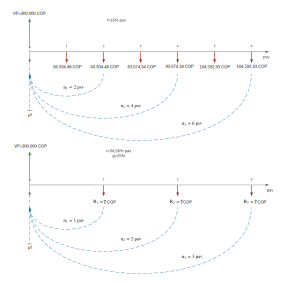
\includegraphics[trim=-78 -5 -78 -5]{7_Capitulo/img/ejemplos/8/8_3.pdf} }   \\ \hline
			%%%%% INICIO FLUJO DE CAJA
			\rowcolor[HTML]{FFB183}
			\multicolumn{2}{|c|}{\cellcolor[HTML]{FFB183}\textbf{4. Declaración de fórmulas}} \\ \hline
			%%%%%%%%%%%%% FIN INSERCIÓN DE IMAGEN
			%%%%%FIN FLUJO DE CAJA
		
			\multicolumn{2}{|c|}{ $VP = \frac{R( (1 + g)^{n} (1+i)^{-n} - 1)}{g-i} $ Valor presente gradiente geométrico}   \\  \hline
			
			%%%%%% INICIO DESARROLLO MATEMÁTICO
			\rowcolor[HTML]{FFB183}
			%%%%%%%%%%INICIO TITULO
			\multicolumn{2}{|c|}{\cellcolor[HTML]{FFB183}\textbf{5. Desarrollo matemático}}       \\ \hline
			%%%%%%%%%% FIN TITULO
			%%%%%%%%%% INICIO MATEMÁTICAS
			\multicolumn{2}{|c|}{  $300.000 \ COP = \frac{R_{1}( (1 + 0,25)^{3} (1+0,3456)^{-3} - 1)}{0,25-0,3456} $}   \\ 
			\multicolumn{2}{|c|}{ $ R_{1} = 225.920,73 \ COP $ }   \\ \hline
			
			%%%%%%%%%% FIN MATEMÁTICAS
			%%%%%% FIN DESARROLLO MATEMÁTICO
			%%%%%% INICIO RESPUESTA
			\rowcolor[HTML]{FFB183}
			%%%%%%%%%%INICIO TITULO
			\multicolumn{2}{|c|}{\cellcolor[HTML]{FFB183}\textbf{6. Respuesta}}   \\ \hline
			%%%%%%%%%% FIN TITULO
			%%%%%%%%%% INICIO RESPUESTA MATEMÁTICA
			\multicolumn{2}{|c|}{ 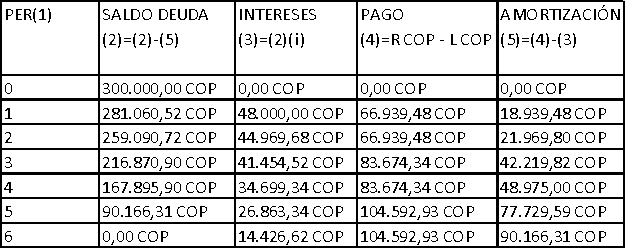
\includegraphics[trim=-78 -5 -78 -5]{7_Capitulo/img/ejemplos/8/8_3_3.pdf} }   \\ \hline
			%\multicolumn{2}{|C{\textwidth}|}{
			%	$R_{58} =  COP  72.478,16(1 + 0,02)^{57} =  COP  224.087,15 $ 
			%}  \\ \hline
			
			
			%%%%%%%%%% FIN MATEMÁTICAS
			%%%%%% FIN RESPUESTA
		\end{longtable}
		%Se crean dos lineas en blanco para que no quede el siguiente texto tan pegado
		%\newline \newline %USARLO SI CREES QUE ES NECESARIO
	\end{center}
 %%%%%%%%%%%%%%%%%%%%%%%%%%FIN EJERCICIO 8c %%%%%%%%%%%%%%%%%%%%%%%%%%%
    %%%%%%%%%%%%%%%%%%%%%%%%%%FIN EJERCICIO 8c %%%%%%%%%%%%%%%%%%%%%%%%%%%

%%%%%%%%%%%%%%%%%%%%%%%%%%FIN EJERCICIO 8 %%%%%%%%%%%%%%%%%%%%%%%%%%%
